\documentclass[border=3pt,tikz,svgnames]{standalone}
\usepackage{tikz}
\usetikzlibrary{decorations.markings,arrows.meta,calc}
\tikzset{>={Stealth[length=1.2mm,width=1.2mm]}}
% 2024 Cambridge brand palette — Crest family.
% Use the brand colours directly (no percent-blends).
\definecolor{Cambridge24LightCrest}{HTML}{FFE2C8}
\definecolor{Cambridge24WarmCrest}{HTML}{FFC392}
\definecolor{Cambridge24Crest}{HTML}{FD8153}
\definecolor{Cambridge24DarkCrest}{HTML}{DD3025}
\colorlet{OrangeFill}{Cambridge24Crest}
\colorlet{OrangeLine}{Cambridge24DarkCrest}

\tikzset{
  DashedArrows/.style 2 args={
    densely dashed, thin,
    postaction={decorate},
    decoration={markings,
      mark=at position #1 with {\arrow{>}},
      mark=at position #2 with {\arrow{>}}
    }
  }
}

\begin{document}

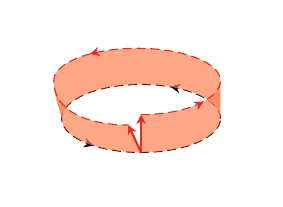
\begin{tikzpicture}[line cap=round]
    \def\Lx{1.44}
    \def\Ly{0.96}
    \path[use as bounding box] (-\Lx,-\Ly) rectangle (\Lx,\Ly);
    \def\Rx{0.7*\Lx}
    \def\Ry{0.45*\Ly}
    \coordinate (O) at (0,-0.2*\Ly);
    \draw[DashedArrows={0.17}{0.62}] (0,-0.2*\Ly) ellipse ({\Rx} and {\Ry});
    \fill[OrangeFill, opacity=0.7] (\Rx,0.3*\Ly) arc(0:-90:{\Rx} and {\Ry}) --++ (0,-0.5*\Ly) arc(-90:0:{\Rx} and {\Ry}) -- cycle;
    \fill[OrangeFill, opacity=0.7] (\Rx,0.3*\Ly) arc(0:180:{1.05*\Rx} and {0.95*\Ry}) -- (-1.1*\Rx,0.3*\Ly) to[out=-90,in=103] (-\Rx,-0.2*\Ly) arc(180:0:{\Rx} and {\Ry}) -- cycle;
    \fill[OrangeFill, opacity=0.7] ($(O)+(0,-\Ry)$) arc(-90:-180:{\Rx} and {\Ry}) to[out=103,in=-90] (-1.1*\Rx,0.3*\Ly) to[out=-90,in=180] ($(O)+(0,-\Ry)+(115:0.4*\Ly)$) -- cycle;

    \draw[OrangeLine, DashedArrows={0.17}{0.62}] ($(O)+(0,0.5*\Ly-\Ry)$) arc(-90:0:{\Rx} and {\Ry}) arc(0:180:{1.05*\Rx} and {0.95*\Ry}) to[out=-90,in=180] ($(O)+(0,-\Ry)+(115:0.4*\Ly)$);

    \draw[OrangeLine, thick, ->] ($(O)+(0,-\Ry)$) --++ (0,0.5*\Ly);
    \draw[OrangeLine, thick, ->] ($(O)+(0,-\Ry)$) --++ (115:0.4*\Ly);
\end{tikzpicture}

\end{document}
